\documentclass[
    bindingoffset=5mm,
    footnoteindent=3mm,
    hyphenation=true
]{template/wut-thesis}

\facultyeiti
\EngineerThesis
\langeng

\graphicspath{{img}}
\addbibresource{bibliography.bib}

\begin{document}

\instytut{Computer Science}
\kierunek{Computer Science}
\specjalnosc{Computer Systems and Networks}
\title{
    General-purpose plotter with control software
}
\poltitle{
    Ploter ogólnego zastosowania z oprogramowaniem sterującym
}
\author{Michał Szopiński}
\album{300182}
\promotor{Maciej Urbański, MSc Eng.}
\date{2022}
\maketitle

\cleardoublepage
\abstract
The goal of this thesis was to construct a general-purpose CNC machine capable
of applying a variety of drawing instruments to a flat surface. The machine
must be easy to set up and utilize by non-tech-savvy users. This is to be
achieved by designing a GUI application that interfaces between the user and the
machine, guiding them through common workflows while keeping the technicalities
to a minimum. The thesis describes the industry conventions on designing and
programming CNC machines, then goes on to describe the designed solution: the
hardware, the firmware, and the control software. The machine was successfully
constructed and tested in practical use-case scenarios. The results of the tests
are presented and discussed in this thesis.

\keywords CNC, microprocessor systems, bare-metal programming, GUI applications

\clearpage
\secondabstract
Tematem pracy dyplomowej jest konstrukcja urządzenia CNC ogólnego zastosowania,
zdolnego do posługiwania się różnymi narzędziami kreślarskimi na płaskich
powierzchniach. Urządzenie to musi być łatwe w instalacji i obsłudze przez
użytkowników nietechnicznych. Wymóg ten należy spełnić poprzez zaprojektowanie
aplikacji graficznej stanowiącej interfejs między użytkownikiem a urządzeniem,
która przeprowadzi go przez realizację powszechnych zadań, jednocześnie
ograniczając zagadnienia techniczne do minimum. Praca opisuje przyjęte standardy
projektowania i programowania urządzeń CNC, a następnie przedstawia opracowane
rozwiązanie: układ elektroniczny (hardware), oprogramowanie układowe (firmware)
oraz oprogramowanie sterujące (software). Urządzenie zostało pomyślnie
skonstruowane i przetestowane pod kątem zdolności do zastosowania w praktyce,
Wyniki testów zostały przedstawione i omówione w niniejszej pracy.

\secondkeywords CNC, systemy mikroprocesorowe, programowanie niskopoziomowe,
aplikacje graficzne


\pagestyle{plain}

\cleardoublepage
\tableofcontents

\cleardoublepage
\pagestyle{headings}

\clearpage
\section{Introduction}

\subsection{CNC machine design}

Computer numerical control (CNC) is a technique which utilizes a computer to
automate the control of a machining tool. By modern definitions, ``machining''
refers to a process in which a material is manipulated to obtain a desired
shape, either through subtractive or additive manufacturing. Machining tools
provide a means to guide a cutting tool along a strictly controlled path
relative to the workpiece, free of human error.

A machining tool with an extensive range of motion in the horizontal plane, but
a limited range of motion in the vertical axis, is commonly called a plotter.
Before the advent of the inkjet printer, these devices were used in engineering
settings to plot functions and draw line art on paper. In modern contexts,
plotters are employed to create inscriptions on rigid or otherwise
unconventional surfaces, where printers may not be used.

In the recent years, CNC machines have been rapidly growing in popularity as
household devices. This is especially true of one such machine, the 3D printer,
which moves a nozzle in three-dimensional space to create a shape out of molten
plastic. As consumers become familiar with CNC technologies, computer-controlled
plotters, drills and lathes may soon become standard workshop equipment.

The concept of numerical control of machining tools is not new; the first
solutions involving punched cards date back to the 1950s. Since that time,
various manufacturers have implemented their own standards for communicating
with machines, the most prominent of which is a data format named G-code.
Originally developed by Gerber Scientific, the format was adopted by many
companies and has become a de-facto industry standard.

In its original form, G-code lacked the ability to read, manipulate and store
data, which made it more akin to a vector graphics description format than to a
programming language. Basic G-code instructions modify the state of the machine
and instruct it to move to a specified position. The machine state impacts the
interpretation of commands and the interpolation between requested positions.

The basic set of instructions enables the operator to (including but not
limited to):
\begin{itemize}
    \item Move in a straight line, draw an arc, or move the tool rapidly
    \item Adjust the movement speed
    \item Switch between absolute and relative positioning
    \item Change the origin of the coordinate system
    \item Switch between metric and US customary units
\end{itemize}
Various manufacturers, however, have opted to implement their own versions of
G-code. This includes differences in instruction encoding, interpretation, and
parsing. Only a small subset of instructions and syntaxes may be expected to
work on all machines universally.

Due to G-code's origin as a vector data format rather than a communication
protocol, there is also no standarized way to obtain any sort of feedback from
the machine to its controlling computer. To establish two-way communication
with the machine, manufacturers employ proprietary solutions.

\subsection{GUI application design}

Modern developments in user interface design show a tendency to step away from
native user controls in favor of web technologies. Desktop and mobile
applications present their interface as an embedded browser window where
controls are implemented using HTML, CSS and JavaScript. This improves user
experience by presenting the user with a modern and familiar UI.

A commonly used software framework for creating this kind of applications is
Electron. It consists of three crucial components:
\begin{itemize}
    \item A standalone JavaScript engine, Node.js. This enables JavaScript to
    be executed outside of a browser context, thanks to which the entire
    application may be written in JavaScript.
    \item JavaScript bindings for native OS functionality, such as interacting
    with the window system or capturing the screen contents. Node.js, being a
    web server by design, lacks this functionality.
    \item A browser context in which the UI code is executed and rendered.
\end{itemize}

When building complex UI applications, it is important to maintain and follow
a strict set of rules regarding data flow and update logic. Between managing
the global program state, handling user interactions and rendering interface
updates, it may be difficult to write readable and maintainable code. A popular
solution to this problem is the React framework, which facilitates the
development of UI applications by introducing the following design principles:
\begin{itemize}
    \item The UI is split into components, each of which is only responsible
    for rendering a small part of the application. Components maintain the
    logical state and handle the side effects of whatever abstraction they
    represent.
    \item Components follow a declarative convention where their rendered
    output is determined solely by their state. This removes the need for
    update logic.
    \item Components can only directly influence components directly contained
    within them. This creates an unidirectional data flow that is easy to manage
    and maintain.
\end{itemize}

\subsection{About this thesis}

The goal of this thesis was to design and to construct a CNC plotter together
with the software needed to control it. The machine implements a subset of the
G-code instruction set that is suitable for general-purpose plotting operations
on flat surfaces. The software is aimed at the consumer market and as such, it
must be easy to set up and use. It is a GUI application which communicates with
the machine over a wired connection.

As part of the project, the following was done:
\begin{enumerate}
    \item A mechanical system capable of moving a drawing instrument in
    three-dimensional space was prepared. The system is a combination of
    pre-made aluminum components and custom-made 3D-printed connector parts.
    \item A microcontroller system was designed to drive stepper motors and to
    communicate with control software. It utilizes ready-made printed circuit
    boards containing driver ICs and the necessary discrete components. A
    custom-made PCB was prepared to house the microcontroller chip together
    with its peripherals.
    \item A firmware program was created to execute CNC instructions and to send
    feedback to control software. It features original code only.
    \item A GUI application was developed to act as an interface between the
    user and the machine. Several common software frameworks were used to
    implement the generic parts of the program.
\end{enumerate}

This thesis is divided into several sections discribing the hardware, the
firmware and the software individually. Each section begins with an analysis
of the relevant project requirements, then goes on to provide a general
overview of the accepted solution, and in the end gives a detailed description
of each major component of the implementation. The final section of this
document contains an analysis of the finished project and drawn conclusions.

Attached to this document is the source code for all described software, the
schematics of the designed microcontroller system and its PCB, and technical
drawings showing the mechanical system.

\clearpage
\section{Theoretical background}

\subsection{CNC machine design}

The concept of numerical control of machining tools is not new; the first
solutions involving punched cards date back to the 1950s. Since that time,
various manufacturers have implemented their own standards for communicating
with machines, the most prominent of which is a data format named G-code.
Originally developed by Gerber Scientific, the format was adopted by many
companies and has become a de-facto industry standard.

In its original form, G-code lacked the ability to read, manipulate and store
data, which made it more akin to a vector graphics description format than to a
programming language. Basic G-code instructions modify the state of the machine
and instruct it to move to a specified position. The machine state impacts the
interpretation of commands and the interpolation between requested positions.

The basic set of instructions enables the operator to (including but not
limited to):
\begin{itemize}
    \item Move in a straight line, draw an arc, or move the tool rapidly
    \item Adjust the movement speed
    \item Switch between absolute and relative positioning
    \item Change the origin of the coordinate system
    \item Switch between metric and US customary units
\end{itemize}
Various manufacturers, however, have opted to implement their own versions of
G-code. This includes differences in instruction encoding, interpretation, and
parsing. Only a small subset of instructions and syntaxes may be expected to
work on all machines universally.

Due to G-code's origin as a vector data format rather than a communication
protocol, there is also no standarized way to obtain any sort of feedback from
the machine to its controlling computer. To establish two-way communication
with the machine, manufacturers employ proprietary solutions.

\subsection{GUI application design}

Modern developments in user interface design show a tendency to step away from
native user controls in favor of web technologies. Desktop and mobile
applications present their interface as an embedded browser window where
controls are implemented using HTML, CSS and JavaScript. This improves user
experience by presenting the user with a modern and familiar UI.

A commonly used software framework for creating this kind of applications is
Electron. It consists of three crucial components:
\begin{itemize}
    \item A standalone JavaScript engine, Node.js. This enables JavaScript to
    be executed outside of a browser context, thanks to which the entire
    application may be written in JavaScript.
    \item JavaScript bindings for native OS functionality, such as interacting
    with the window system or capturing the screen contents. Node.js, being a
    web server by design, lacks this functionality.
    \item A browser context in which the UI code is executed and rendered.
\end{itemize}

When building complex UI applications, it is important to maintain and follow
a strict set of rules regarding data flow and update logic. Between managing
the global program state, handling user interactions and rendering interface
updates, it may be difficult to write readable and maintainable code. A popular
solution to this problem is the React framework, which facilitates the
development of UI applications by introducing the following design principles:
\begin{itemize}
    \item The UI is split into components, each of which is only responsible
    for rendering a small part of the application. Components maintain the
    logical state and handle the side effects of whatever abstraction they
    represent.
    \item Components follow a declarative convention where their rendered
    output is determined solely by their state. This removes the need for
    update logic.
    \item Components can only directly influence components directly contained
    within them. This creates an unidirectional data flow that is easy to manage
    and maintain.
\end{itemize}

\clearpage
\section{Analysis of market-available solutions}

\subsection{HP 7470A}

Although no longer popular, plotters used to be a commonly found piece of office
equipment. Designed to connect to a personal computer, they were used to plot
graphics before inkjet printers became available. One such plotter is the
Hewlett-Packard 7470A, introduced in 1982.

The 7470A used a felt-tip pen to draw monochrome graphics on A4 paper.
Communication was established over an RS-232 serial connection, and it used a
proprietary language called HP-GL to encode vector data. Software for the device
was often written in BASIC. Its task was to generate HP-GL instructions from
input data according to hard-coded algorithms \cite{7470a}.

The HP-GL language offered capabilities similar to those of G-code, while also
defining a protocol for serial communication required to obtain feedback from
the device. A handshake procedure was employed to govern the transmission of
data, so as not to overflow the machine's serial buffer.

Functionally, the machine was capable of:
\begin{itemize}
    \item Moving freely in the horizontal plane, raising and lowering the
    pen
    \item Drawing lines and arcs
    \item Drawing text using multiple fonts
    \item Scaling and translating output coordinates
    \item Switching between unit systems
    \item Switching between absolute and relative coordinates
    \item Moving at different speeds
\end{itemize}
The above list fully encompasses the features of standard G-code, but also it
makes the machine useful without the need for dedicated control software. The
7470A could be hand-operated from a simple serial terminal.

\subsection{LinuxCNC}

A more modern CNC solution is LinuxCNC, a software suite designed to bypass the
control firmware of a CNC machine and to interact with the machine's hardware
directly. By using a real-time Linux kernel and communicating over the
high-speed PCI bus, the software makes it possible to control stepper motors
with a personal computer \cite{linuxcnc}.

Not being linked to any manufacturer gives LinuxCNC the freedom to accept any
data format and to directly execute arbitrary toolpath generation algorithms.
Nonetheless, the software implements its own G-code parser with a wide range of
functionality equivalent to that of commercial manufacturers. Features include:
\begin{itemize}
    \item Linear and rotational axes of motion
    \item Additional toolpath curves
    \item Rotation and translation of the coordinate system
    \item Compensation for tool size during movement
    \item Canned cycles for lathes and drills
    \item Multiple tools
\end{itemize}

Being a purely software solution, the system allows the user to inspect the
CNC machine state in great detail. The user may step through a CNC program and
view generated toolpaths before and after they are executed. Current parameters
of the machine, including its configuration, position and memory state, are
displayed on-screen.

\clearpage
\section{CNC machine design}

\subsection{Project requirements}

The goal of this project is to construct a general-purpose CNC machine capable
of applying a variety of drawing instruments to a flat surface. This involves
the capability to freely move a tool in three-dimensional space, with a large
range of motion in the horizontal plane and a relatively restricted range of
motion in the vertical axis. It must be compatible with common workpiece
formats, including A4 paper. It must have the ability to use interchangeable
tools of different shapes and sizes.

Because the machine does not face much physical resistance during normal
operation, there is no need to monitor the tool position - it may be assumed
that it is in accordance with the executed instructions. As such, an open-loop
control scheme may be implemented. Similarly, because the machine is not used
to remove material from the workpiece, it may operate at a pre-defined constant
feed rate, low enough for open-loop control.

To achieve partial compatibility with other solutions available on the market,
it must use G-code as the input instruction format, and it must implement a
large enough subset of G-code to implement basic functionality. This includes:
\begin{enumerate}
    \item Three types of motion: rapid, linear and arc
    \item Absolute and incremental coordinate mode
    \item Metric and Imperial units of measurement
    \item Commands and syntax related to feed rate, even though the
    functionality itself is not implemented
\end{enumerate}

The machine uses a serial port to communicate with its controlling computer.
Because modern personal computers do not come with a physical RS-232 serial
port, the connection must be established over USB, using generic drivers to
create a virtual serial port.

To enhance user experience, the machine must provide feedback in response to
input. The feedback includes:
\begin{enumerate}
    \item The current physical coordinates of the work tool, sent periodically
    \item A message sent whenever a commands starts or finishes executing
    \item An error code describing any syntax or semantic errors in the command
    \item An interpretation of the currently executing command, including:
        \begin{itemize}
            \item The type of movement it triggered
            \item The source and destination of the movement
            \item The center of the arc, in the case of arcs
        \end{itemize}
\end{enumerate}

Table~\ref{projectRequirements} contains a summary of the requirements
of the CNC machine.

\begin{table}[ht]
    \begin{center}
        \begin{tabular}{ |l|c|c| }
            \hline
            Parameter & Value & Unit \\
            \hline
            Axes of motion & 3 & - \\
            Controller type & Open-loop & - \\
            Input method & G-code over serial port & - \\
            Connection interface & USB & - \\
            Supported motion types & Rapid, linear, arc & - \\
            X axis travel & 200 & mm \\
            Y axis travel & 200 & mm \\
            Z axis travel & 5 & mm \\
            Max tool diameter & 18 & mm \\
            Max workpiece width & 297 & mm \\
            \hline
        \end{tabular}
        \caption{Project requirements of the CNC machine}
        \label{projectRequirements}
    \end{center}
\end{table}

The machine must be user-friendly. It must come with control software which
guides the user through common use-case scenarios. These scenarios are:
\begin{enumerate}
    \item Batch execution, where the user specifies a file containing
    instructions to be executed in sequence
    \item Command prompt, where the user may type commands by hand and observe
    their effects
    \item Bitmap tracing, where the user submits a raster image to be converted
    into a vector approximation, which can then be drawn by the machine
\end{enumerate}

The software must allow the user to select which serial port to use. It detects
the presence of the CNC machine on the other end informs the user if a
connection problem occurs. During program execution, the user may view each
command, see its execution status, its associated error message, and a graphical
representation of the motion it initiated.

\clearpage
\subsection{Hardware}

\subsubsection{Mechanics}

\begin{figure}[ht]
    \begin{center}
        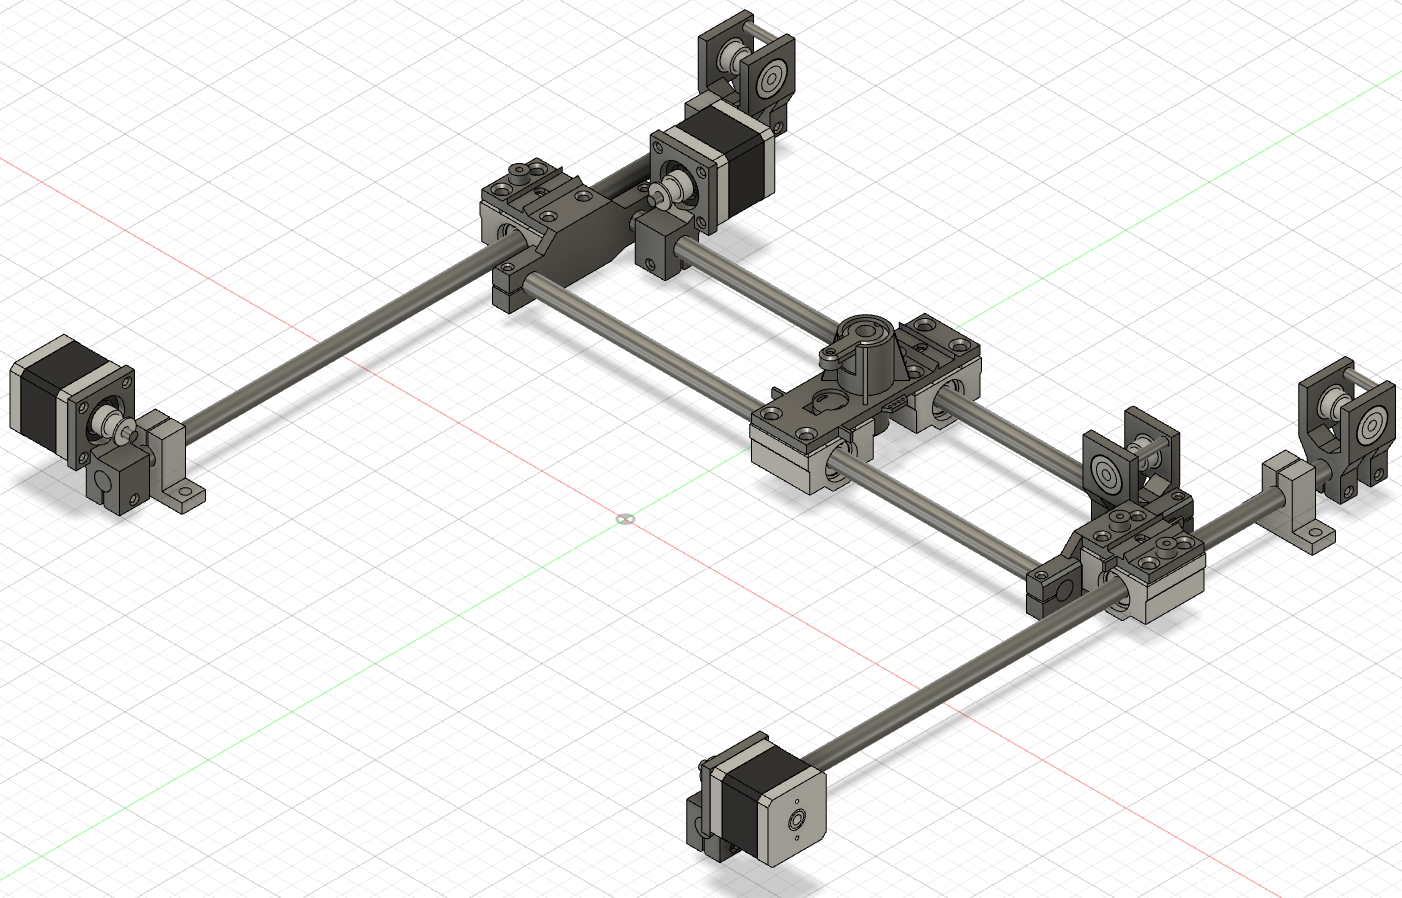
\includegraphics[width=\linewidth]{mechanics_overview}
        \caption{A 3D model of the mechanics.}
    \end{center}
\end{figure}

The CNC machine consists of a set of moving platforms and cylindrical rails
mounted atop an 8-millimeter sheet of acrylic. It contains custom 3D-printed
parts used to join prefabricated metal components. The parts were designed in
Fusion 360 and printed with an Anycubic Photon S printer using the SLA
printing technology.

Bolted directly to the base are two parallel rails, set 350 mm apart, which
guide movement in the Y axis. On each of the rails, mounted on top of a linear
bearing, is a platform which provides a mounting point for another pair of
rails. This pair, set 54 mm apart, guides movement in the X axis.

Placed across the second pair of rails, also mounted on linear bearings, is the
head assembly. It houses the interchangeable head, which holds the drawing
instrument, and guides its movement in the Z axis. It also provides a mounting
point for a small stepper motor coupled with the head.

Movement in the XY plane is driven by three stepper motors, coupled with their
respective platforms by timing belts. This enables movement at large speeds
while providing a reasonable amount of precision. Movement in the Z axis is
achieved with a leadscrew-type mechanism, where a small stepper motor with a
threaded shaft moves the head up and down.

\begin{figure}[ht]
    \centering
    \begin{minipage}{0.5\textwidth}
        \centering
        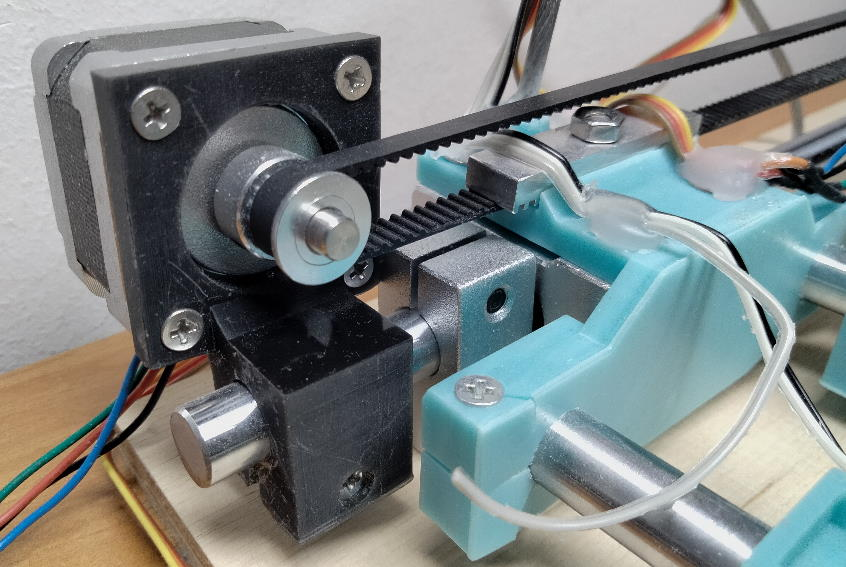
\includegraphics[width=0.9\textwidth]{xy_drive}
        \caption{XY drive using a timing belt.}
    \end{minipage}\hfill
    \begin{minipage}{0.5\textwidth}
        \centering
        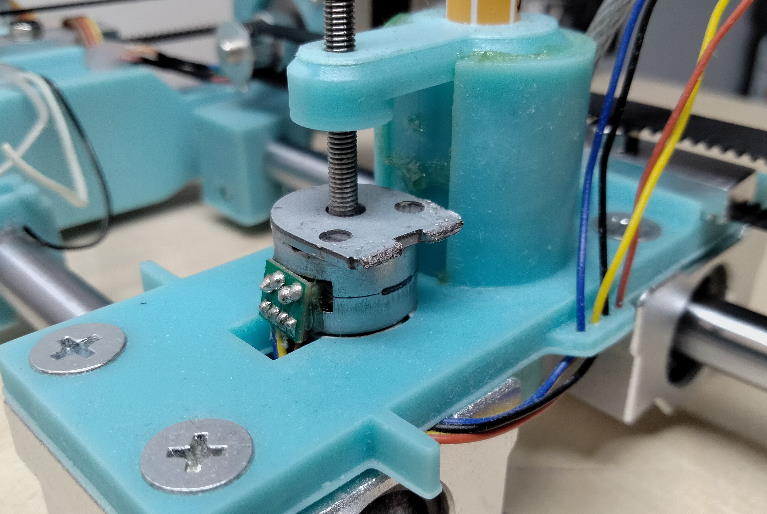
\includegraphics[width=0.9\textwidth]{z_drive}
        \caption{Z drive using a leadscrew.}
    \end{minipage}
\end{figure}

The stepper motor used for XY movement is a JK35HY28-0504, a bipolar stepper
motor commonly used for CNC applications. It consumes 0.5 A per coil and
provides a torque of 0.1 Nm \cite{jk35hy28}. The smaller stepper motor used for
Z-axis movement is a generic no-brand bipolar motor available from online
retailers. It has been measured to provide sufficient torque at 0.2 A per coil.

The mechanical system described above is sufficient to achieve a full range of
motion in all three axes. Four stepper motors with a maximum current consumption
of 3.4 A may be controlled to achieve any toolpath. A microcontroller system,
shown in figure~\ref{fig:schematic}, was designed to perform this task. The
circuit schematic and its corresponding PCB were created in KiCad.

\clearpage
\begin{sidewaysfigure}[ht]
    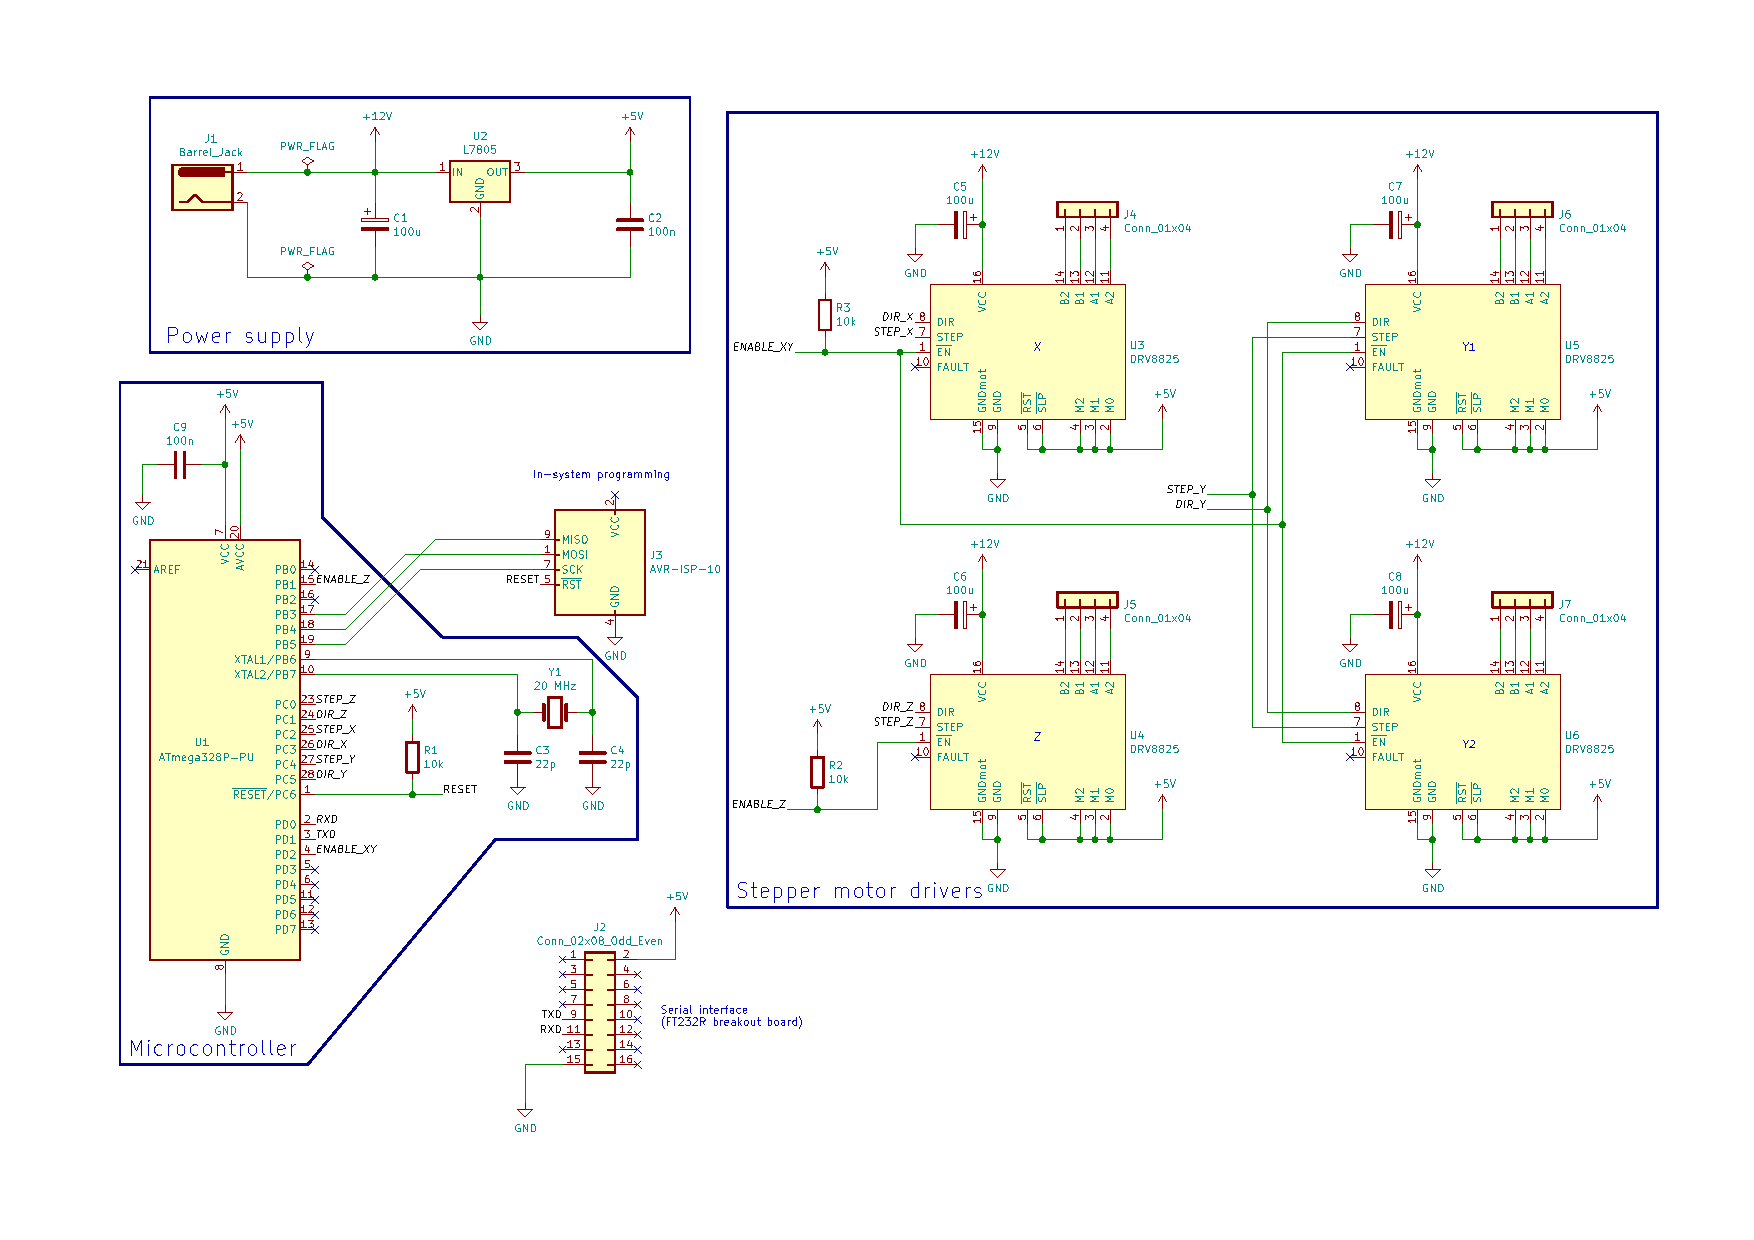
\includegraphics[width=\linewidth]{schematic}
    \caption{A schematic of the microcontroller system.}
    \label{fig:schematic}
\end{sidewaysfigure}

\clearpage

\subsubsection{Motor drivers}

Driving the stepper motors is delegated to a separate sub-circuit based on the
DRV8825. The DRV8825 is an integrated circuit which comes with its own power
regulation, the ability to adjust coil current, adjustable-resolution
microstepping, and a built-in indexer \cite{drv8825}. Controlling a motor is
thus reduced to choosing a direction through the $DIR$ pin and strobing The
$STEP$ pin with the appropriate timing. To save energy, coils may be deenergized
using the $\overline{EN}$ pin.

In the circuit, there are four DRV8825 circuits, one for each motor. They are
connected directly to the high-voltage power rail, which is used to power both
the motors and the IC logic. A large 100 {\textmu}F decoupling capacitor is
placed near the power pin, in accordance with manufacturer recommendations.

The chips are premanently configured to use the maximum microstepping resolution
available, 1/32. This improves the resolution of the CNC machine and
reduces mechanical noise. $\overline{EN}$ pins are connected to pullup
resistors, which prevents motor coils from being energized before the
microcontroller has booted.

\subsubsection{Microcontroller system}

At the center of the system lies an ATmega328p, a very popular microcontroller
manufactured by Microchip Technology. It was chosen partially due to its
ubiquity and a large amount of resources available online. Below is an overview
of its parameters.

\begin{table}[ht]
    \begin{center}
        \begin{tabular}{ |l|c| }
            \hline
            Parameter & Value \\
            \hline
            Architecture & 8-bit AVR \\
            Throughput & 20 MIPS at 20 MHz \\
            Program memory & 32 KB \\
            SRAM & 2 KB \\
            I/O pin count & 23 \\
            Timers & 3 timers with compare mode \\
            Hardware USART & Yes \\
            Hardware USB & No \\
            In-system programming & Yes \\
            Operating voltage & 1.8 to 5.5 V \\
            \hline
        \end{tabular}
        \caption{Parameters of the ATmega328p \cite{atmega328p}}
    \end{center}
\end{table}

What makes the ATmega328p suitable for this application is the number of I/O
pins, multiple hardware timers and a hardware USART transmitter-receiver.
It also features in-system programming (ISP) capabilities, which enable fast
prototyping without having to remove the chip from the circuit board. A major
disadvantage is the low maximum clock frequency and an 8-bit architecture, which
may limit the speed of curve calculations.

The microcontroller is powered from the +5V rail, which is provided by a LM7805
linear voltage regulator. A decoupling capacitor is installed for a stable
operation. Clock signal is generated by an on-board crystal oscillator, which
uses a quartz crystal connected to two of the pins. A pullup resistor prevents
the MCU from resetting, unless the reset pin is pulled low by an ISP programmer.

Although the chip lacks USB capabilities, a serial connection via USB may
be established through external circuitry. In this case, a socket is provided
for a breakout board housing the FT232R USB-to-UART integrated circuit.
Royalty-free drivers provided by the manufacturer enable serial communication
by means of a virtual serial port \cite{ft232}.

\subsubsection{Printed circuit board}

A printed circuit board was designed based on the above schematic. It is a
two-layer board where the bottom layer is used as a ground plane. Figures
\ref{pcb} and \ref{pcb_photo} show the details of the design.

\begin{figure}[ht]
    \begin{center}
        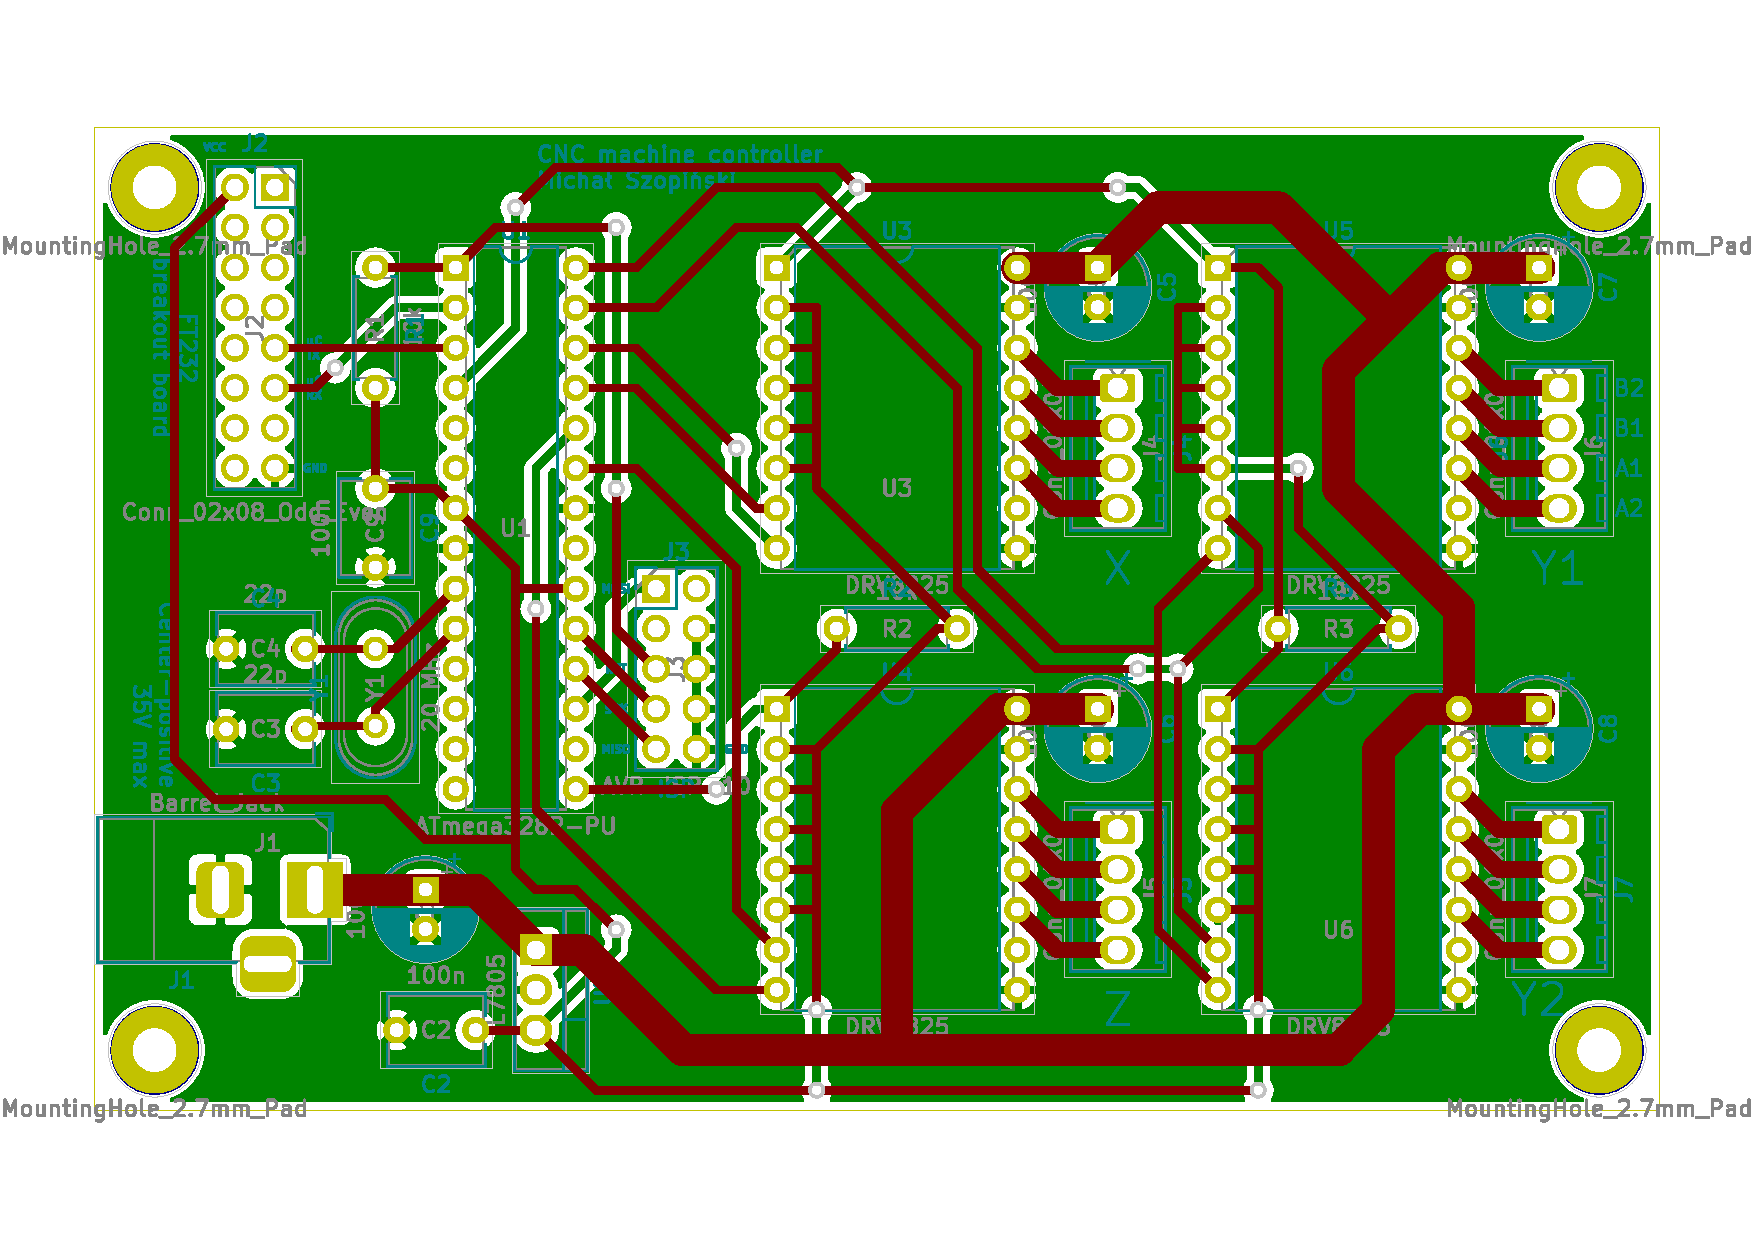
\includegraphics[width=1\linewidth]{pcb}
        \caption{A schematic of the designed PCB.}
        \label{pcb}
    \end{center}
\end{figure}
\begin{figure}[ht]
    \begin{center}
        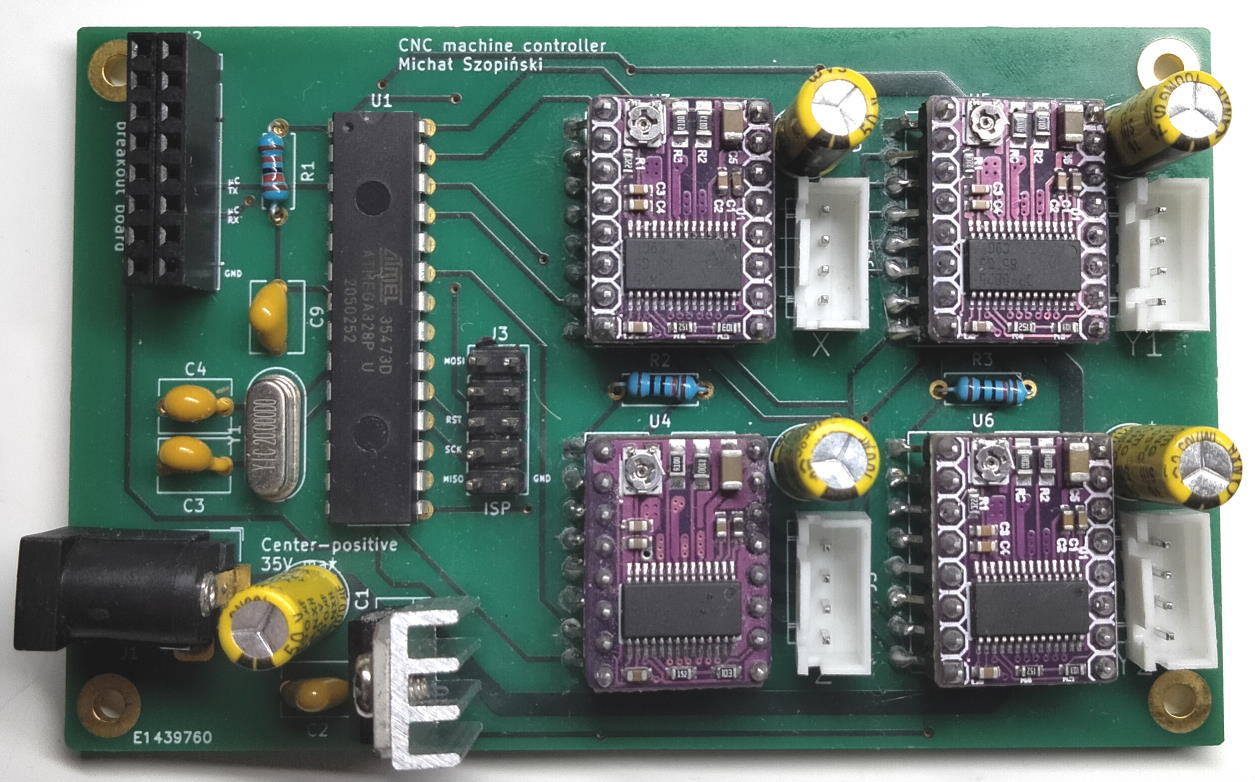
\includegraphics[width=1\linewidth]{pcb_photo}
        \caption{The designed PCB, assembled.}
        \label{pcb_photo}
    \end{center}
\end{figure}
\clearpage

\clearpage
\section{Firmware}

\clearpage
\subsection{Software}

\begin{figure}[ht]
    \begin{center}
        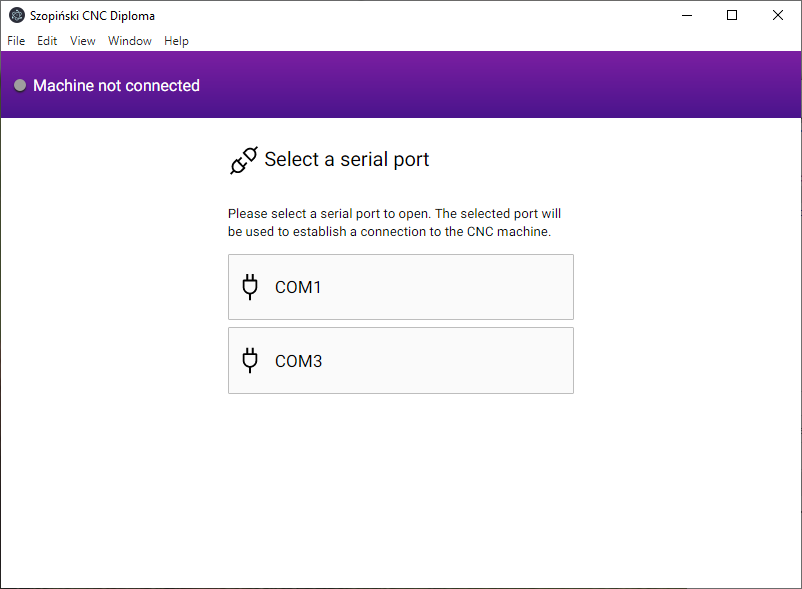
\includegraphics[width=0.75\linewidth]{serialselect}
        \caption{Serial port selection screen of the control software.}
        \label{serialselect}
    \end{center}
\end{figure}

The control software is implemented using Electron, a framework for writing
desktop applications using web technologies. This allows it to present an
elegant, modern user interface while retaining the ability to perform low-level
operations such as serial communication. It also makes it easy to achieve
cross-platform compatibility.

Electron applications are written in JavaScript. They consist of a main process,
which interacts with the operating system, and a renderer process, which
displays the user interface in a browser window and exchanges information with
the main process. This ensures security in case the renderer process becomes
compromised.

Web development practices favor the use of externally developed software to
solve commonly encountered problems. Such software is distributed in the form of
packages and installed by a package manager. Every project has a list of
dependencies which must be collected before it is run.

The following libraries and tools were used to create this application:

\begin{itemize}
    \item Yarn, a combined package manager and project manager. Used for
    managing dependencies and launching build utilities.
    \item Webpack, a module bundler. Needed to compile the project into a
    compact set of files suitable for consumption by Electron.
    \item React, a framework for building user interfaces. It introduces a
    system of components and a mechanism to coordinate the flow of information
    within the application.
    \item React Redux, a library for managing the global application state.
    Facilitates handling events which impact multiple unrelated parts of the
    user interface.
    \item React Router, a library to handle screen navigation.
    \item Node SerialPort, a JavaScript wrapper around the operating system's
    serial interface.
    \item Sass, a dialect of CSS which introduces a hierarchical structure.
    \item ESLint, a code analysis tool for detecting errors and enforcing code
    style.
\end{itemize}

Because the application does not fetch data from the Internet nor does it
execute code from the file system, the renderer process is allowed to interact
with the operating system directly. This simplifies program design by removing
the need to communicate with the main process. The main process is thus reduced
to boilerplate code which opens the browser window and loads an HTML document
containing the application.

\subsubsection{Global program state}

\begin{figure}[ht]
    \begin{center}
        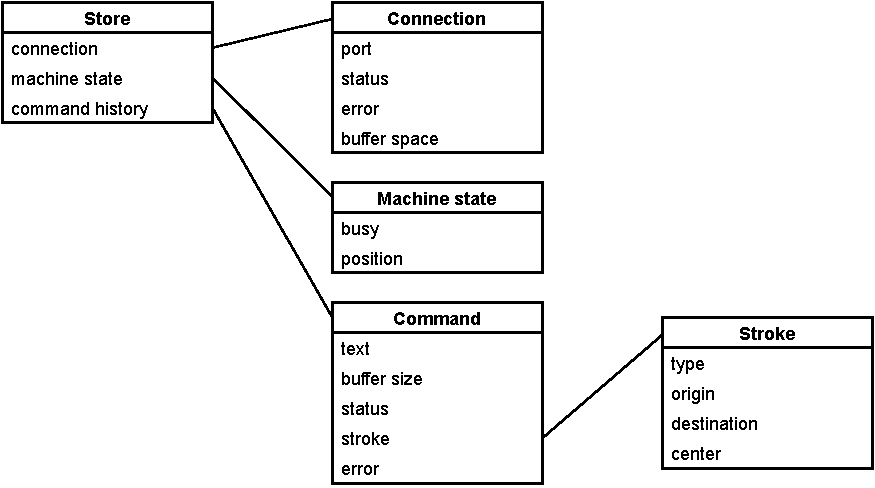
\includegraphics[width=0.75\linewidth]{globalstate}
        \caption{Structure of the store.}
        \label{store}
    \end{center}
\end{figure}

Main program functionality is centered around the global state object, which
by Redux terminology is referred to as the \textit{store}. Redux introduces the
following design principles \cite{redux}:
\begin{enumerate}
    \item The store may only be changed by dispatching \textit{actions}, which
    may be thought of as events. Actions are dispatched in response to user
    interaction or incoming or outgoing serial traffic. Actions are handled
    by \textit{reducer} functions, which dictate how they impact the store.
    \item Changes in the store may be \textit{subscribed to} by various
    components of the program. When subscribers detect that a relevant part
    of the store has changed, they may trigger appropriate behavior.
\end{enumerate}

The store is divided into three top-level objects (figure~\ref{store}):
connection state, machine state, and command history. Changes to the connection
state cause the program to establish or to close a serial connection. The
machine state object reflects feedback received from the device, and is observed
by the user interface. The command history object governs data transmission
to the device and allows the user to monitor the execution of commands.

\subsubsection{Serial communication}

\begin{figure}[ht]
    \begin{center}
        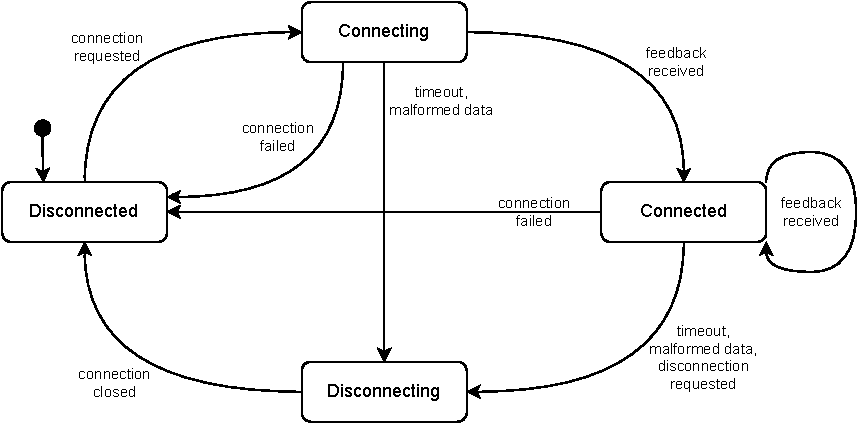
\includegraphics[width=0.75\linewidth]{serialstate}
        \caption{State transition of the serial connection.}
        \label{serialstate}
    \end{center}
\end{figure}

A global store subscriber is registered to handle serial communication. When the
user first launches the application, they are presented with a serial port
selection screen (figure~\ref{serialselect}). Choosing one of the options
changes the connection status to \texttt{connecting}. The subscriber detects
this change and attempts to establish a new serial connection.

The device sends three kinds of feedback. The software verifies that the
feedback is received within a certain time frame and that it isn't malformed.
Violating the serial protocol terminates the connection. Receiving valid
feedback marks the connection as established (see figure~\ref{serialstate}).

There are three kinds of feedback:

\begin{itemize}
    \item Position feedback, sent every quarter second. Receiving this packet
    updates the store's machine state and establishes the connection.
    \item ``Command started'' feedback, sent once a command has been executed
    but before its motion has finished. Contains an interpretation of the
    command by the machine's G-code parser. Receiving this packet updates
    the command history and triggers an attempt to send commands to the device
    (see next section).
    \item ``Command finished'' feedback, sent once the motion initiated by a
    command has finished or if there was no motion. Updates the command history.
\end{itemize}

\subsubsection{Command history and queue}
\label{sending}

\begin{figure}[ht]
    \begin{center}
        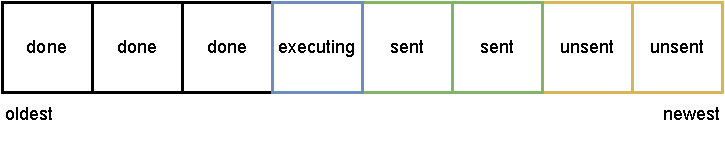
\includegraphics[width=0.6\linewidth]{commandhistory}
        \caption{Lifecycle of commands within the command history.}
        \label{commandhistory}
    \end{center}
\end{figure}

In order to maintain a logical connection between sent commands and received
feedback, the application maintains a global command history object to
coordinate the exchange of data between the software and the firmware
(see figure~\ref{commandhistory}).

A command begins its lifecycle when a \texttt{sendCommand} action is dispatched.
The new command, whose status is \texttt{unsent}, is placed at the end of the
command history. The serial communication subscriber observes the history and
attempts to send the command, provided there are no other sent commands.

The device's receive buffer is limited in size and cannot handle an overflow
condition. For this reason, the software keeps track of the amount of available
buffer space and delays the transmission of commands as necessary. If the
command's content, encoded as UTF-8, is within this limit, the command is sent.
Its status is set to \texttt{sent} and its size is subtracted from the
available buffer space.

Once sent, the command is read and executed by the machine. When feedback
arrives, the command is marked as \texttt{executing}, its interpretation and
error code are updated, and its size is added back to the buffer space.
This prompts an attempt to send more commands.

Finally, once the command has been executed, its status is set to \texttt{done}.
Executed commands are purged from the history when no longer relevant to the
user.

\clearpage
\begin{figure}[ht]
    \begin{center}
        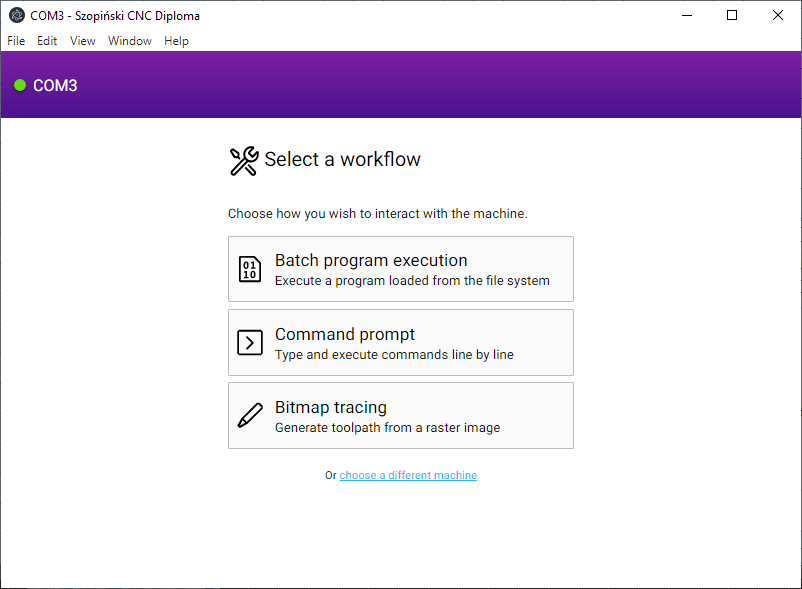
\includegraphics[width=0.8\linewidth]{workflowselect}
        \caption{Workflow selection screen.}
        \label{workflow}
    \end{center}
\end{figure}
\begin{figure}[ht!]
    \begin{center}
        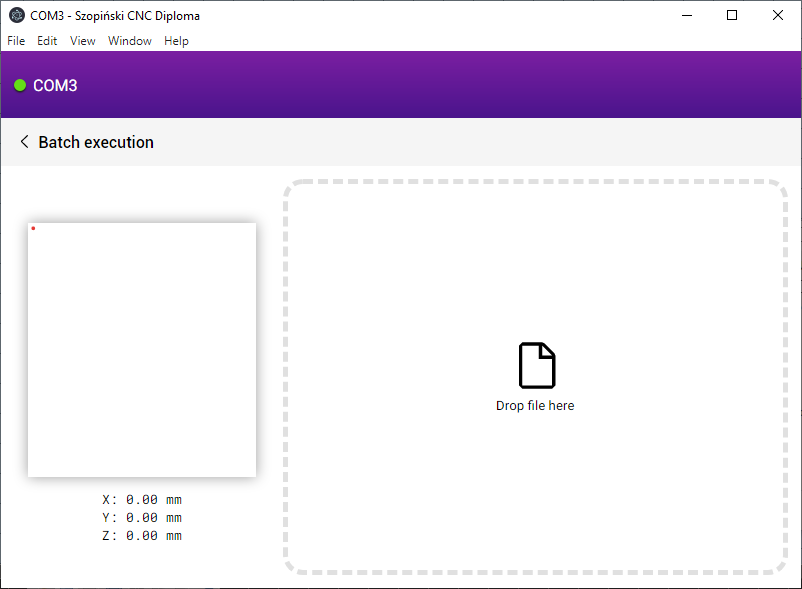
\includegraphics[width=0.8\linewidth]{batch}
        \caption{Batch execution screen, before dropping a file.}
    \end{center}
\end{figure}

\clearpage
\begin{figure}[ht]
    \begin{center}
        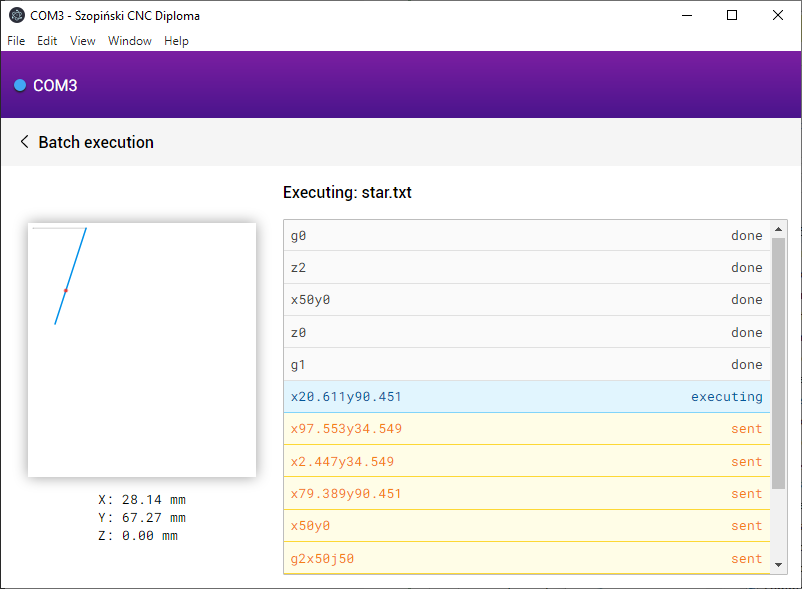
\includegraphics[width=0.8\linewidth]{batchexecuting}
        \caption{Batch execution screen, during execution.}
        \label{batch}
    \end{center}
\end{figure}
\begin{figure}[ht!]
    \begin{center}
        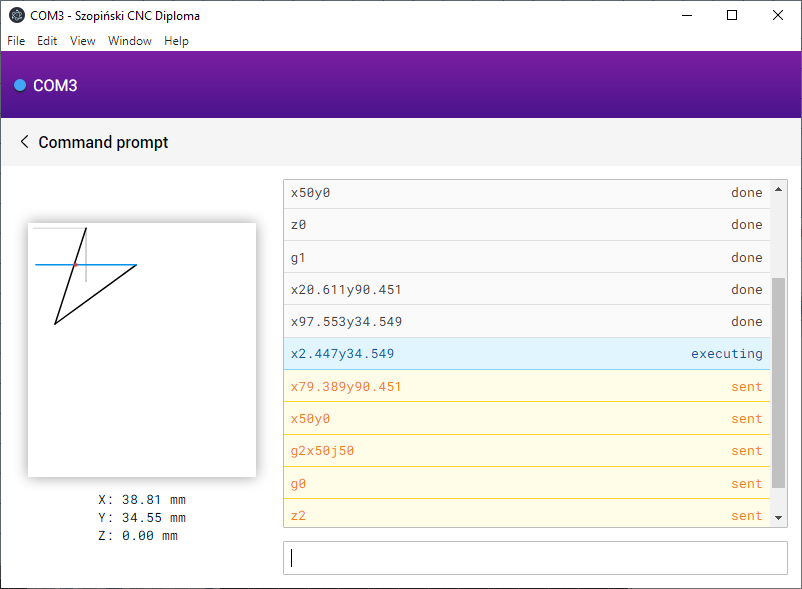
\includegraphics[width=0.8\linewidth]{commandprompt}
        \caption{Command prompt screen.}
        \label{commandprompt}
    \end{center}
\end{figure}

\clearpage
\subsubsection{Motion preview}

When the application is launched, the user is presented with a workflow
selection screen (figure~\ref{workflow}). They may choose from three different
workflows: batch execution, command prompt and bitmap tracing. The first two
screens are simple interfaces exposing the functionality described in
section~\ref{sending}.

In each screen, the user may view a list of executing commands and a preview
of the motion initiated by them (figures~\ref{batch} and~\ref{commandprompt}).
The preview is generated by translating motion interpretation objects
(received as feedback from the machine) into SVG tags embedded directly in the
HTML document.

Translating linear motion is trivial. The SVG \texttt{line} element takes
arguments specifying an origin and a destination, which are given directly.
Rapid motion requires additional calculations for checking if it should be
split into two lines (as depicted in figure~\ref{rapid}). Translating circular
motion, however, is more complicated.

\begin{figure}[ht]
    \begin{center}
        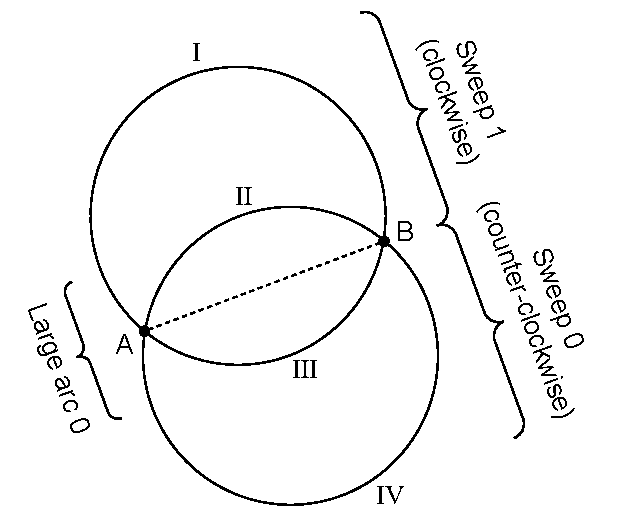
\includegraphics[width=0.4\linewidth]{arcflag}
        \caption{Four ways to draw an arc given two points and a radius.}
        \label{arcflag}
    \end{center}
\end{figure}

In SVG, there are two ways to describe arcs. Full arcs may be drawn using the
\texttt{circle} element, which takes a radius and a center point. Partial
arcs can only be drawn with the \texttt{path} element and its \texttt{A}
instruction \cite{circles}. Because there are multiple paths through which two
points may be connected by an arc (figure~\ref{arcflag}), the \texttt{A}
instruction takes several arguments:

\begin{itemize}
    \item Implicit arc origin, $x_{orig}$ and $y_{orig}$
    \item $x$-axis radius $R_x$ and $y$-axis radius $R_y$
    \item $x$-axis rotation $\theta$
    \item Large arc flag $f_L$
    \item Sweep flag $f_S$
    \item Arc end, $x_{dest}$ and $y_{dest}$
\end{itemize}

The translation starts by calculating the radius. For circular arcs, the
$x$-axis radius and the $y$-axis radius are equal:
\begin{equation*}
    R_x = R_y = \sqrt{(x_{dest} - x_{center})^2 + (y_{dest} - y_{center})^2}
\end{equation*}
If the origin and the destination are the same, a \texttt{circle} element is
rendered and the calculation ends. Otherwise, the remaining arc parameters are
computed.

$x$-axis rotation $\theta$ is irrelevant for circles, therefore it is always
assigned a value of $0$. The sweep flag $f_S$ is conceptually equvialent to
drawing the arc in a clockwise or a counter\-clockwise manner, and so its value
is inferred from the motion type.
\begin{align*}
    \theta = 0 &&
    f_S = \begin{cases}
        1 & \text{for clockwise arcs} \\
        0 & \text{for counter-clockwise arcs}
    \end{cases}
\end{align*}

The large arc flag $f_L$ may be calculated by converting the origin and
destination points to polar coordinates relative to the arc center and measuring
the angular distance $\Delta$. If $\Delta$ exceeds $180\degree$, the arc is
large (figure~\ref{arctravel}).
\begin{gather*}
    \alpha = \text{atan2}(y_{orig} - y_{center}, x_{orig} - x_{center}) \\
    \beta = \text{atan2}(y_{dest} - y_{center}, x_{dest} - x_{center})
\end{gather*}
\begin{align*}
    \begin{aligned}
        \Delta_{cw} = \begin{cases}
            \beta - \alpha & \text{if } \alpha < \beta \\
            2\pi - \alpha + \beta & \text{otherwise}
        \end{cases} \\
        \Delta_{ccw} = \begin{cases}
            2\pi - \beta + \alpha & \text{if } \alpha < \beta \\
            \alpha - \beta & \text{otherwise}
        \end{cases}
    \end{aligned}
    &&
    f_L = \begin{cases}
        1 & \text{if } \Delta > \pi \\
        0 & \text{otherwise}
    \end{cases}
\end{align*}

\begin{figure}[ht]
    \begin{center}
        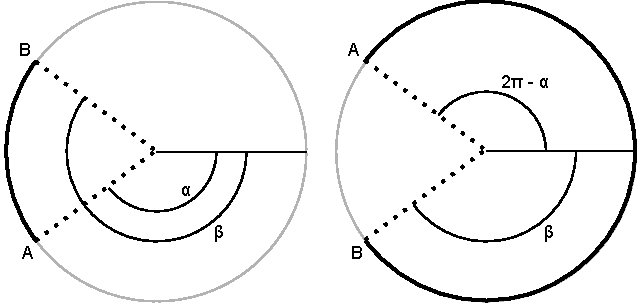
\includegraphics[width=0.6\linewidth]{arctravel}
        \caption{Measuring angular distance for clockwise arcs.}
        \label{arctravel}
    \end{center}
\end{figure}

\clearpage
\subsubsection{Bitmap tracing}

\begin{figure}[ht]
    \begin{center}
        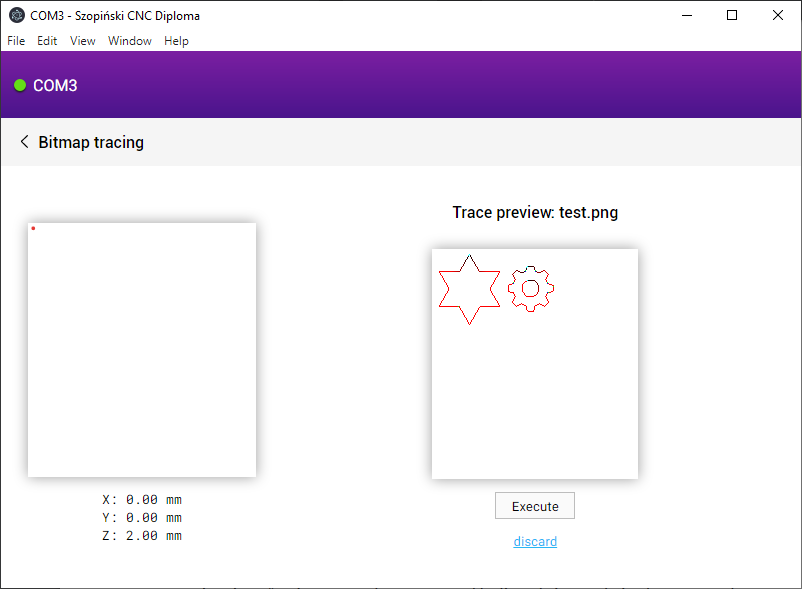
\includegraphics[width=0.75\linewidth]{trace}
        \caption{Bitmap tracing screen.}
        \label{trace}
    \end{center}
\end{figure}

A major feature which makes the software user-friendly is bitmap tracing,
which takes a raster image and converts it to a sequence of G-code commands.
After the user uploads an image, they are presented with a preview of the
generated toolpath. They may execute the generated commands or discard the
result (figure~\ref{trace}).

Raster images contain no information about the curves they depict, however, a
vector approximation of an image may be constructed by linearly interpolating
between each marked pixel. A continuous sequence of points that may be drawn
without raising the tool is referred to as a \textit{segment}. Bitmap tracing
is implemented in five steps:
\begin{enumerate}
    \item Bitmap normalization, where the bitmap is reduced to a basic form
    \item Segment discovery, where continuous sequences of points are found
    \item Segment extension, where neighboring segments are connected
    \item Linear reduction, where unnecessary segment points are removed
    \item G-code generation, where segments are translated into commands
\end{enumerate}

Tracing begins by normalizing the input bitmap's dimensions and pixel data. The
bitmap is expanded to match the work area's aspect ratio. Transparency is
removed by superimposing the bitmap over a white background. Colors are
quantized such that if no channel R, G or B exceeds the value 127, a pixel
is made black, otherwise it is made white (figure~\ref{normalize}).

\clearpage
\begin{figure}[ht]
    \centering
    \begin{minipage}{0.5\textwidth}
        \centering
        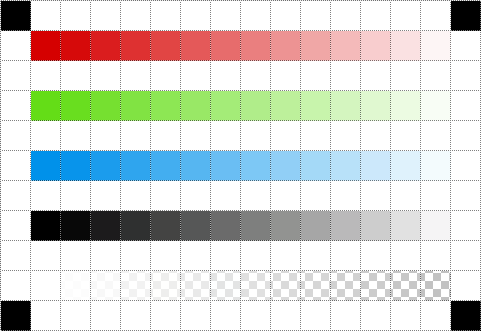
\includegraphics[width=0.5\textwidth]{normaltestin}
        \caption{Image before normalization.}
    \end{minipage}\hfill
    \begin{minipage}{0.5\textwidth}
        \centering
        
\includegraphics[width=0.5\textwidth]{normaltestout}
        \caption{Image after normalization.}
        \label{normalize}
    \end{minipage}
\end{figure}

Once the bitmap has been normalized, segment discovery begins. The bitmap is
scanned left-to-right, top-to-bottom in search of unexplored black pixels.
When such a pixel is encountered, it becomes the starting point of a new
segment. The program then attempts to include as many points in the segment as
possible, given certain constraints (figure~\ref{segments}).

\begin{figure}[ht]
    \begin{center}
        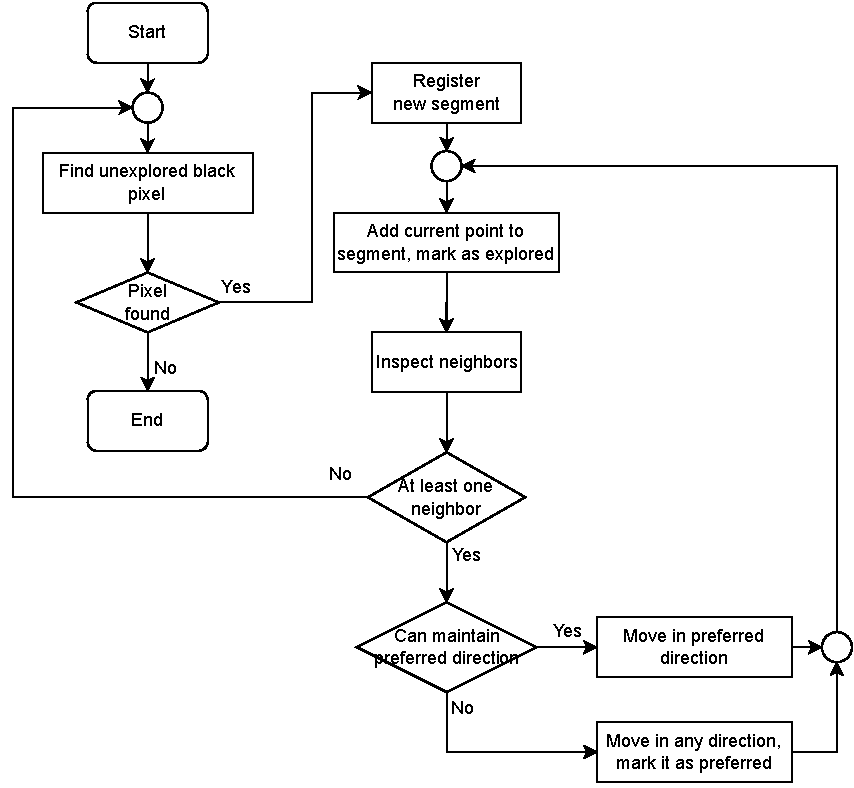
\includegraphics[width=0.6\linewidth]{segments}
        \caption{Flowchart of segment discovery and exploration.}
        \label{segments}
    \end{center}
\end{figure}

On every iteration of the segment exploration algorithm, neighbors of the most
recently added pixel are inspected. If there are no neighbors elegible for
inclusion in the segment, the segment is terminated and the algorithm returns
to the scanning phase. This ensures that all pixels are eventually included in
a segment.

If there are multiple neighbors elegible for inclusion in a segment, the
algorithm gives preference to the one which maintains the current direction of
travel (figure~\ref{straight}). This reduces the amount of generated commands
by allowing multiple points to be covered by a single line.

\begin{figure}[ht]
    \begin{center}
        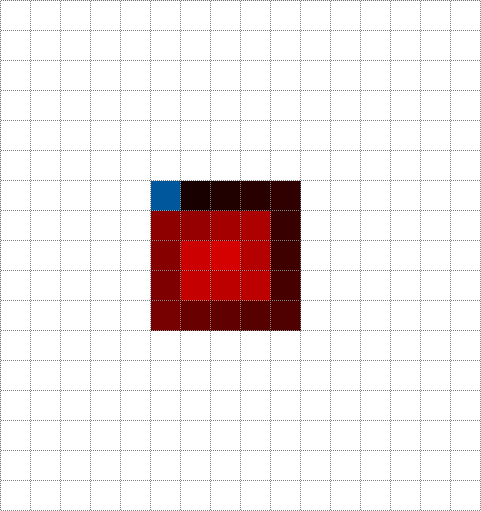
\includegraphics[width=0.25\linewidth]{straightpreview}
        \caption{Trace preview of a solid black square. Blue denotes segment
        origin, black-to-red gradient denotes segment progression.}
        \label{straight}
    \end{center}
\end{figure}


Segments constructed in the described manner contain interpolations between
their constituent points, but not between other segments. To enable the
construction of more complex shapes, segments that neighbor other segments are
extended to maintain continuity. Segments whose terminal points neigbor each
other are extended to form loops.

Before segments are translated to G-code, an optimization is performed where
linear sequences are reduced to their terminal points. For each point of each
segment, if the following holds:
\begin{align*}
    \big(x - x_{prev} = x_{next} - x\big)
    \land
    \big(y - y_{prev} = y_{next} - y\big)
\end{align*}
then the point is eliminated.

Finally, G-code commands are generated from each segment. The machine makes a
rapid move to the initial point of a segment, lowers the tool, and then linearly
moves from one point to another. Once all segments have been drawn, the machine
returns to the coordinate origin.

\clearpage
\section{Tests and verification}

Described in this section is a test suite intended to verify that the designed
hardware, firmware and software behave correctly and meet project requirements.
Because the three components are heavily co-dependent, conducting pure unit
tests would require the development of dedicated simulation software. This has
not been done as part of the thesis; as such, this test suite depends on all
components functioning correctly at the same time.

\subsection{Hardware tests}

The hardware must:
\begin{enumerate}
    \item Support microcontroller operation when supplied with 12 volts
    \item Be programmable through ISP
    \item Establish communication over USB
    \item Drive all stepper motors correctly
\end{enumerate}

The prined circuit board presented in section~\ref{pcbsection} was set up as
shown in figure~\ref{pcbsetup}. Power was supplied from an benchtop power
supply. Current consumption on power-up was 30 mA and the transmit LED blinked
every quarter second, indicating that the microcontroller is functioning
properly and sending feedback.

\begin{figure}[ht]
    \centering
    \begin{minipage}{0.5\textwidth}
        \centering
        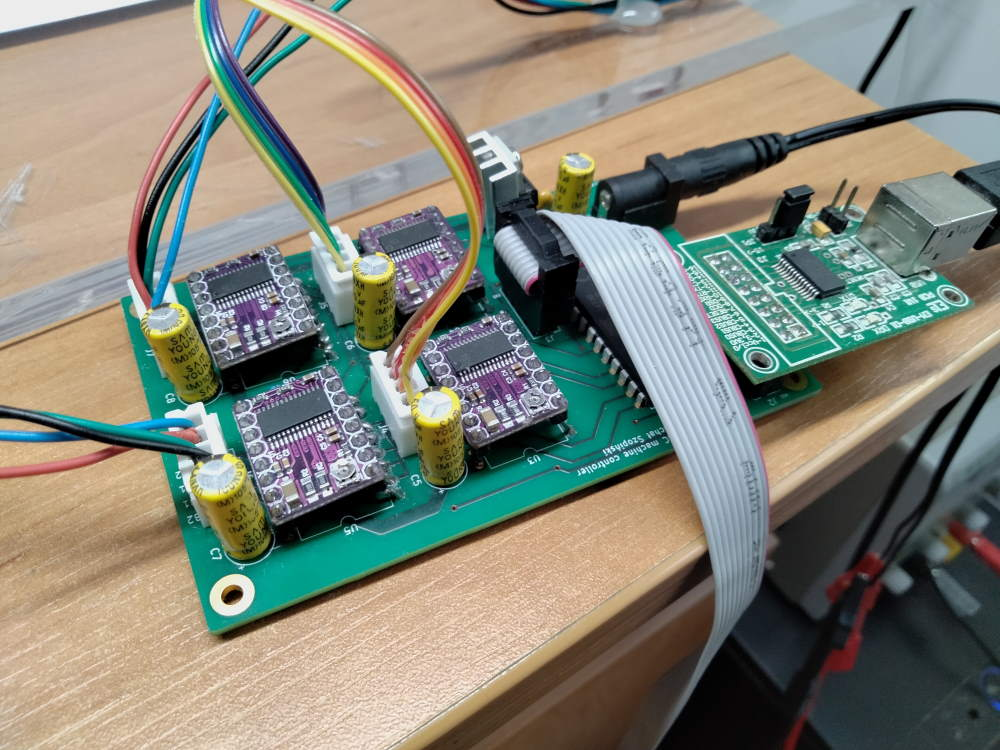
\includegraphics[width=0.9\textwidth]{pcbsetup}
        \caption{PCB set-up.}
        \label{pcbsetup}
    \end{minipage}\hfill
    \begin{minipage}{0.5\textwidth}
        \centering
        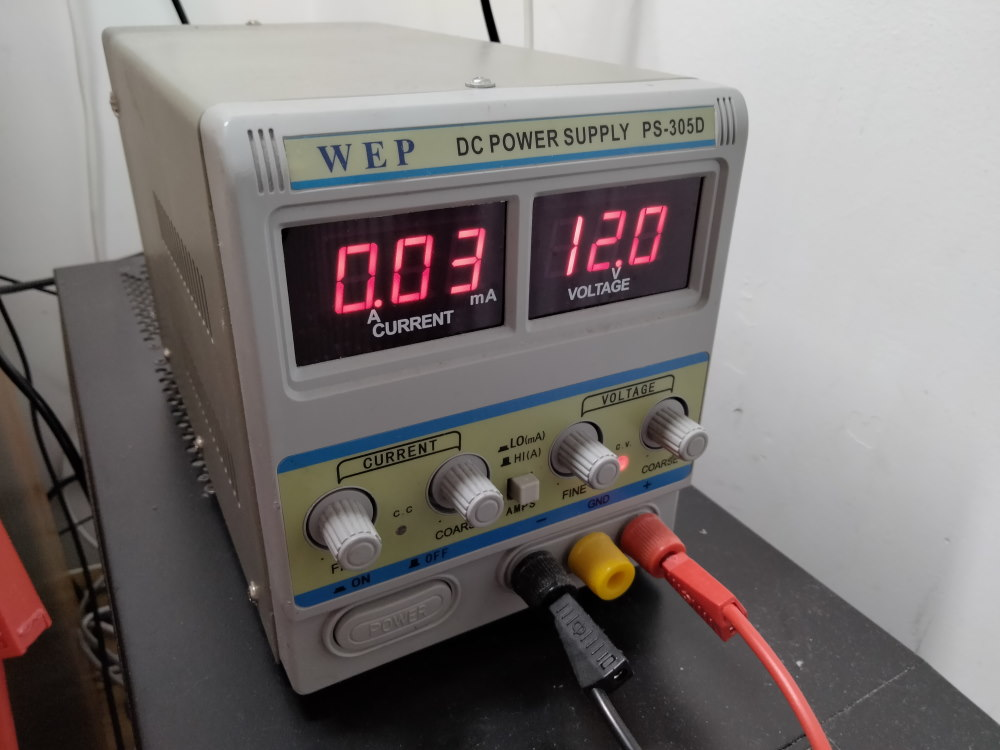
\includegraphics[width=0.9\textwidth]{current}
        \caption{Initial current consumption.}
        \label{current}
    \end{minipage}
\end{figure}

A USBasp programmer was connected to the ISP port to verify the device's
in-system programming capability. An attempt to upload the firmware binary was
successful. Opening the device's virtual serial port in a terminal emulator
revealed the structure of the periodically sent feedback
(figure~\ref{feedback}).

Issuing several \texttt{G0} commands initiated rapid movement. All motors were
driven correctly. The machine moved smoothly in all three axes.

\begin{figure}[ht]
    \begin{center}
        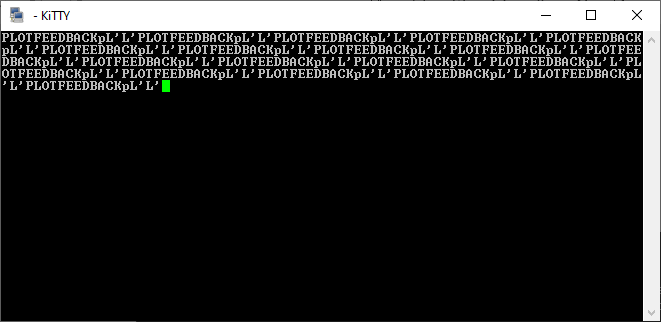
\includegraphics[width=0.6\textwidth]{feedback}
        \caption{Feedback data viewed in a terminal.}
        \label{feedback}
    \end{center}
\end{figure}

\subsection{Firmware tests}

Because the firmware issues feedback in a human-unreadable binary form, all
tests of the firmware were conducted through the control software's command
prompt. The software provides a way to inspect the received feedback and gain
insight into the way the firmware operates.

The firmware must:
\begin{enumerate}
    \item Read and parse commands
    \item Provide periodic feedback describing the machine's current position
    \item Provide feedback on the execution of commands, including their
    interpretation
    \item Handle and provide diagnostics for syntax and semantic errors in
    commands
    \item Support rapid, linear and arc motion
    \item Support commands for switching between absolute and relative
    coordinates
    \item Support commands for changing the units of measurement
\end{enumerate}

\subsubsection{Command parsing and feedback}

When the device was first powered on, periodic feedback was observed in the
terminal window. For the purpose of this test, the control software was modified
to display a human-readable representation of the feedback. The machine sent
data describing its position (figure~\ref{posfeedback}) and the interpretation
of commands it received (figure~\ref{comfeedback}).

\clearpage
\begin{figure}[ht]
    \centering
    \begin{minipage}{0.5\textwidth}
        \centering
        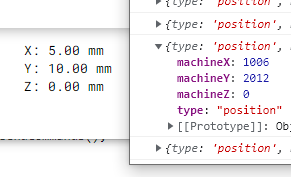
\includegraphics[width=0.9\textwidth]{positionfeedback}
        \caption{Position feedback, raw data and conversion to millimeters.}
        \label{posfeedback}
    \end{minipage}\hfill
    \begin{minipage}{0.5\textwidth}
        \centering
        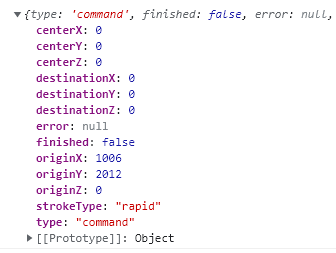
\includegraphics[width=0.9\textwidth]{commandfeedback}
        \caption{Command feedback.}
        \label{comfeedback}
    \end{minipage}
\end{figure}

The firmware's ability to parse and validate syntax was tested. Several commands
were issued testing various productions of the command language
(figure~\ref{syntax}). The parser correctly handles G-code words with decimals,
comments, command deletion and line number markers. Errors are reported when
the parser encounters syntax errors and unsupported features: parameter
settings, unimplemented word letters, unimplemented G-word numbers.

\begin{figure}[ht]
    \begin{center}
        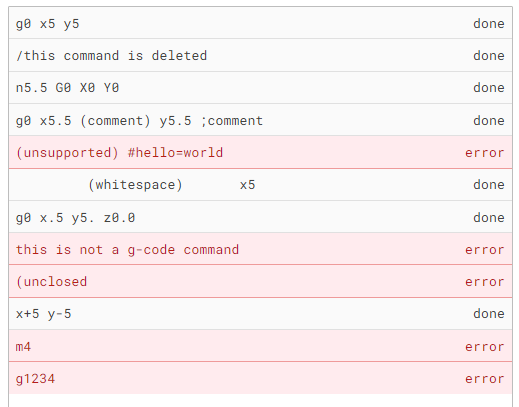
\includegraphics[width=0.6\textwidth]{syntax}
        \caption{Commands correctly parsed by the firmware.}
        \label{syntax}
    \end{center}
\end{figure}

\subsubsection{Command execution}

Two G-code files were prepared to demonstrate the machine's ability to execute
rapid, linear and arc movement. The machine successfully executed the commands
and drew geometric patterns on paper (figure~\ref{lineararc}). A series of
commands was prepared to test modal G-codes. The machine behaved as intended
(figure~\ref{modals}).

\begin{figure}[ht]
    \begin{center}
        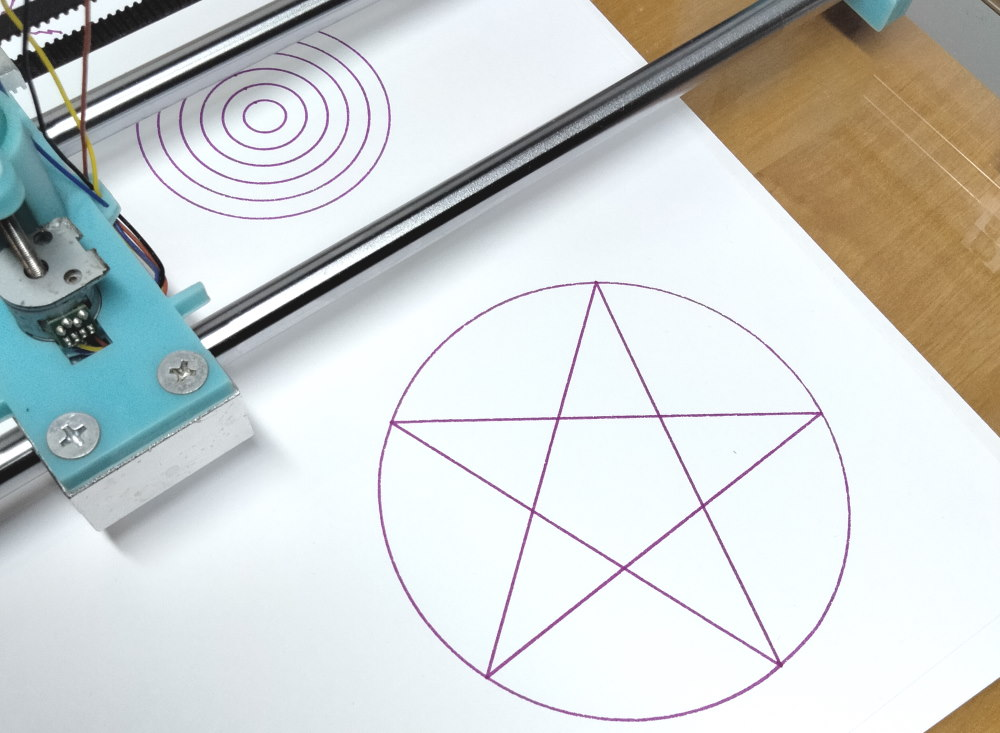
\includegraphics[width=0.8\textwidth]{lineararc}
        \caption{Lines and arcs drawn by the machine.}
        \label{lineararc}
    \end{center}
\end{figure}

\begin{figure}[ht]
    \begin{center}
        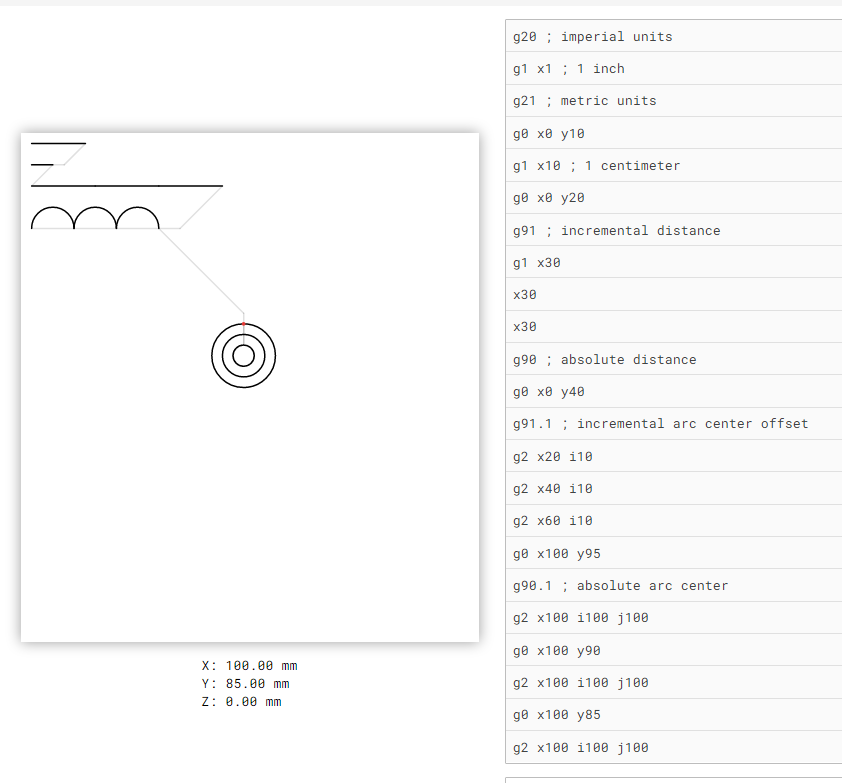
\includegraphics[width=0.8\textwidth]{modal}
        \caption{Modal commands and their impact on command execution. Preview
        drawn based on interpretation data from the machine.}
        \label{modals}
    \end{center}
\end{figure}

\clearpage
\subsection{Software tests}

The software's ability to perform basic tasks (connect to the machine,
send and receive commands) has largely been verified in the previous sections.
This section verifies the remaining major components of the user experience.

The software must be able to:
\begin{itemize}
    \item Establish connections and handle connection errors
    \item Keep track of sent commands and display feedback to the user
    \item Generate a preview of motion initiated by the commands
    \item Trace bitmaps
\end{itemize}

\subsubsection{Connectivity}

When the application is launched, the user is presented with a serial port
selection screen. Selecting a port prompts an attempt to establish a connection.
The machine has been verified to correctly handle the following error
conditions:
\begin{enumerate}
    \item Connection failures -- verified by disconnecting the device's power
    supply
    \item Feedback timeouts -- verified by holding the microcontroller in reset
    state
    \item Malformed feedback -- verified by resetting the microcontroller
    mid-transmission
\end{enumerate}
An error dialog is displayed and the software returns to the port selection
screen (figure~\ref{connfailed}).

\begin{figure}[ht]
    \begin{center}
        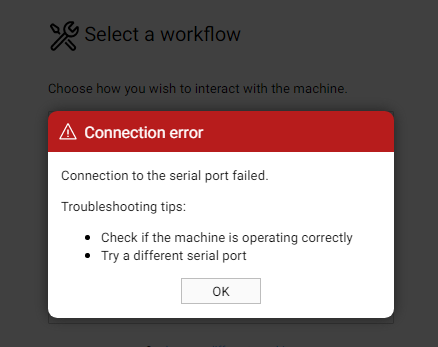
\includegraphics[width=0.6\textwidth]{connfailed}
        \caption{``Connection failed'' dialog.}
        \label{connfailed}
    \end{center}
\end{figure}

A status bar is displayed throughout the application. Its value is correctly
updated to match the current state of the connection (figure~\ref{status}).

\begin{figure}[ht]
    \begin{center}
        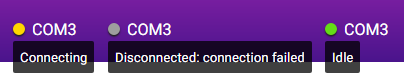
\includegraphics[width=0.6\textwidth]{status}
        \caption{Different values of the status bar.}
        \label{status}
    \end{center}
\end{figure}

\subsubsection{Command list and preview}

The command list component, displayed by every workflow screen, reflects the
state of the command queue. By attempting to send multiple long commands in a
row, the buffer overflow prevention mechanism discussed in section~\ref{sending}
may be observed.

The commands are displayed properly (figure~\ref{commandlist}). Their status is
shown to the right of the command text and they are color-coded. Errors may be
viewed by hovering over the ``Error'' label. The command list scrolls
automatically so that the currently executing command is always in the middle.

\begin{figure}[ht]
    \begin{center}
        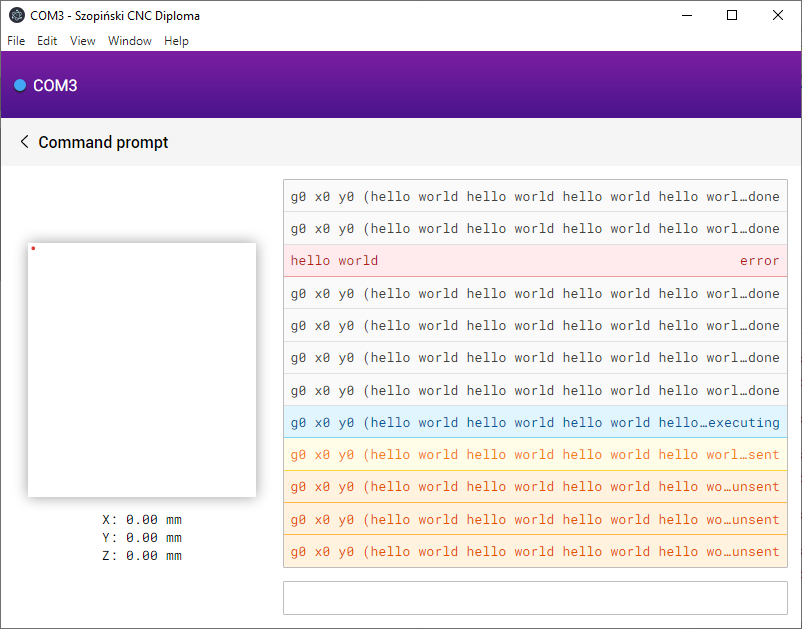
\includegraphics[width=0.5\textwidth]{commandlist}
        \caption{Command list showing commands at different lifecycle stages.}
        \label{commandlist}
    \end{center}
\end{figure}

Command preview has been verified to correctly display motion interpretations
by preparing a sequence of commands generating rapid movement, linear movement,
circles and arcs (figure~\ref{commandpreview}).

\begin{figure}[ht]
    \begin{center}
        
\includegraphics[width=0.2\textwidth]{commandpreview}
        \caption{Command preview showing different types of curves.}
        \label{commandpreview}
    \end{center}
\end{figure}

\subsubsection{Bitmap tracing}

To verify that the bitmap feature is behaving correctly, a test bitmap was
prepared (figure~\ref{heloworin}) which contains the following features:
\begin{itemize}
    \item Simple isolated segments
    \item Neighboring segments
    \item Loops
    \item Intersecting diagonal lines
    \item Light-colored areas and transparent areas
    \item Sigle-pixel segments, isolated and connected
    \item Filled-in areas
    \item Freehand shapes
\end{itemize}
Figure~\ref{helowor} shows the result of the trace. Simple segments (the
\texttt{L} shape) are drawn correctly. Segments which neighbor other segments
(\texttt{H}, \texttt{E}) are extended to preserve continuity. Loops are closed
(\texttt{O}). Light and transparent areas are ignored. Linear segments are
reduced to a single command.

Examining the filled-in area reveals the algorithm's tendency to travel in a
straight path. The area is entered through the top-left corner and a long broken
line is drawn. Later, the remaining area is revisited and a maze-like structure
is created. Figure~\ref{helowortrace} shows the path taken by the algorithm.

\begin{figure}[ht]
    \begin{minipage}{0.5\textwidth}
        \centering
        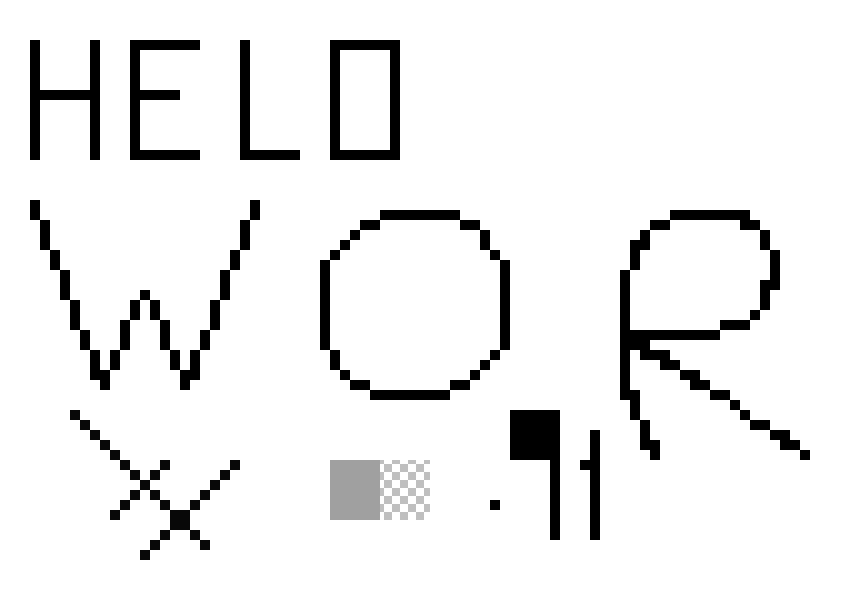
\includegraphics[width=0.9\textwidth]{heloworin}
        \caption{Test bitmap for tracing.}
        \label{heloworin}
    \end{minipage}\hfill
    \begin{minipage}{0.5\textwidth}
        \centering
        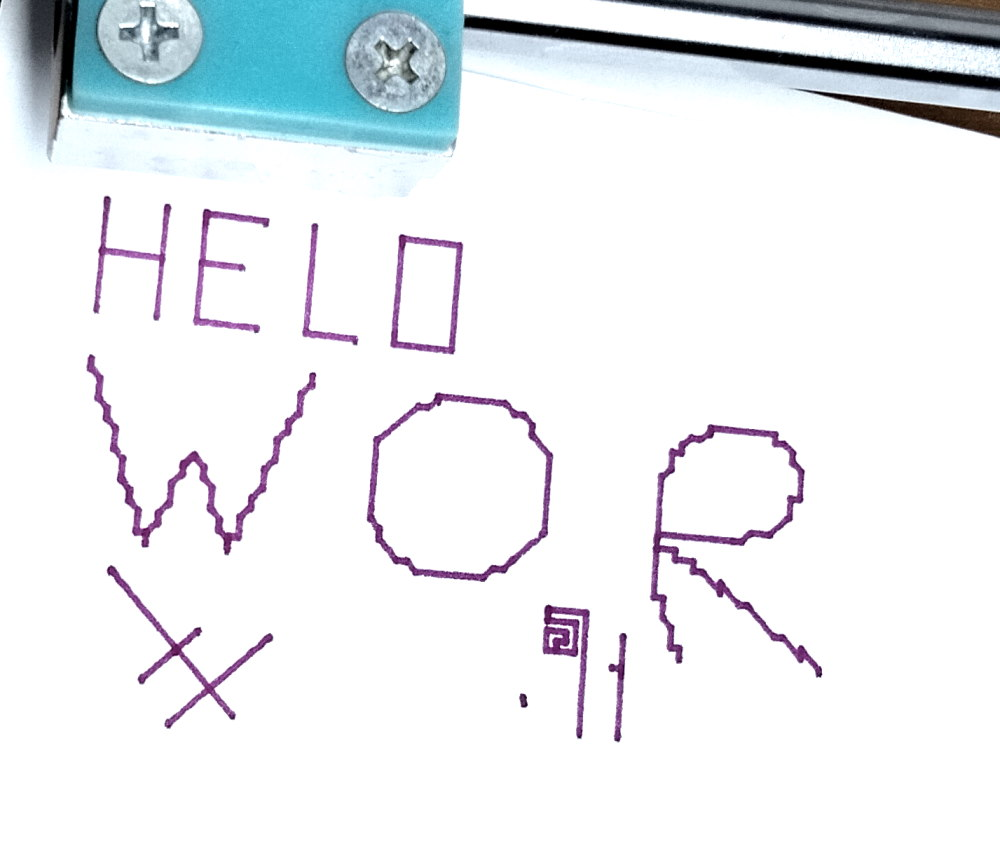
\includegraphics[width=0.9\textwidth]{helowor}
        \caption{Result of the trace.}
        \label{helowor}
    \end{minipage}
    \begin{minipage}{0.5\textwidth}
        \centering
        
\includegraphics[width=0.6\textwidth]{helowortrace}
        \caption{Trace preview.}
        \label{helowortrace}
    \end{minipage}
\end{figure}

To test the machine's capabilities to the fullest extent, a large bitmap
consisting mostly of filled-in areas was supplied to the bitmap tracing
algorithm. The resulting toolpath is shown in figure~\ref{kicad}.

Maze-like structures are can be seen throughout the picture. As the drawing
progresses, imperfections start to appear - the tip of the drawing instrument
becomes offset in the Y axis by about a millimeter.

This is likely not an issue in the firmware or the software, but rather a fault
in the 3D-printed part which holds the tool. The part is given too much
clearance relative to the tube which holds it, and may become tilted when
drawing long vertical lines. A solution to this problem was planned, but it
could not be implemented in a timely manner.

\begin{figure}[ht]
    \begin{center}
        
\includegraphics[width=0.9\textwidth]{kicad}
        \caption{A general test of the plotter's ability to draw traced
        bitmaps.}
        \label{kicad}
    \end{center}
\end{figure}

\clearpage
\section{Summary}


\cleardoublepage
\printbibliography
\clearpage

\pagestyle{plain}
\listofappendicestoc
Below is a list of appendices to the thesis:
\begin{itemize}
    \item Source code for the project firmware and software
    \item A schematic of the circuit and the printed circuit board
    \item A 3D model of the mechanical system with custom-made parts
\end{itemize}
A compact disc containing the appendices is attached.


\end{document}
